\documentclass[12pt]{article}
\usepackage[margin=2.5cm]{geometry}
\usepackage{enumerate}
\usepackage{amsfonts}
\usepackage{amsmath}
\usepackage{fancyhdr}
\usepackage{amsmath}
\usepackage{amssymb}
\usepackage{amsthm}
\usepackage{mdframed}
\usepackage{graphicx}
\usepackage{subcaption}
\usepackage{adjustbox}
\usepackage{listings}
\usepackage{xcolor}
\usepackage{booktabs}
\usepackage[utf]{kotex}
\usepackage{hyperref}
\usepackage{accents}

\definecolor{codegreen}{rgb}{0,0.6,0}
\definecolor{codegray}{rgb}{0.5,0.5,0.5}
\definecolor{codepurple}{rgb}{0.58,0,0.82}
\definecolor{backcolour}{rgb}{0.95,0.95,0.92}

\lstdefinestyle{mystyle}{
    backgroundcolor=\color{backcolour},
    commentstyle=\color{codegreen},
    keywordstyle=\color{magenta},
    numberstyle=\tiny\color{codegray},
    stringstyle=\color{codepurple},
    basicstyle=\ttfamily\footnotesize,
    breakatwhitespace=false,
    breaklines=true,
    captionpos=b,
    keepspaces=true,
    numbers=left,
    numbersep=5pt,
    showspaces=false,
    showstringspaces=false,
    showtabs=false,
    tabsize=1
}

\lstset{style=mystyle}

\pagestyle{fancy}
\renewcommand{\headrulewidth}{0.4pt}
\lhead{CSC 343}
\rhead{Worksheet 9 Solution}

\begin{document}
\title{CSC343 Worksheet 9 Solution}
\maketitle

\bigskip

\begin{enumerate}[1.]
    \item \textbf{Exercise 11.1.1:}

    \bigskip

    \begin{enumerate}[a)]
        \item

    \begin{center}
    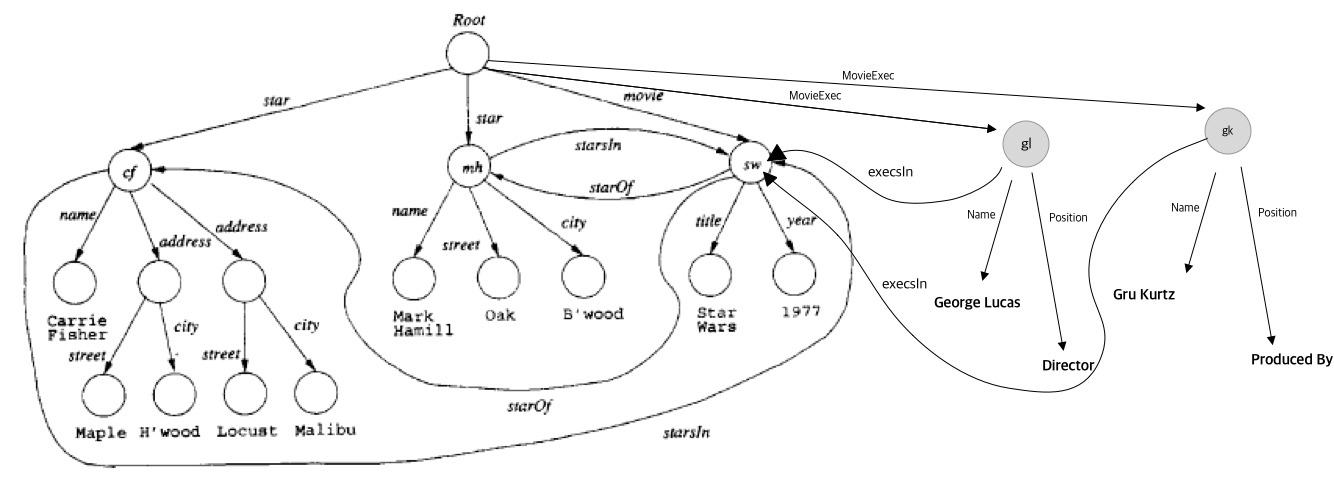
\includegraphics[width=\linewidth]{images/worksheet_9_solution_4.png}
    \end{center}

        \bigskip

        \underline{\textbf{Notes:}}

        \begin{itemize}
            \item Semistructured data
            \begin{itemize}
                \item serves as a model suitable for \textbf{databases integration}, that is,
                for describing the data contained in two or more databases that contain similar data with
                different schemas

                \item It serves as the underlying model for notations such as XML, to be taken
                up in Section 2, that are being used to share information on the web.
            \end{itemize}

            \item Semistructured Data Representation
            \begin{itemize}
                \item is a collection of nodes

            \begin{center}
            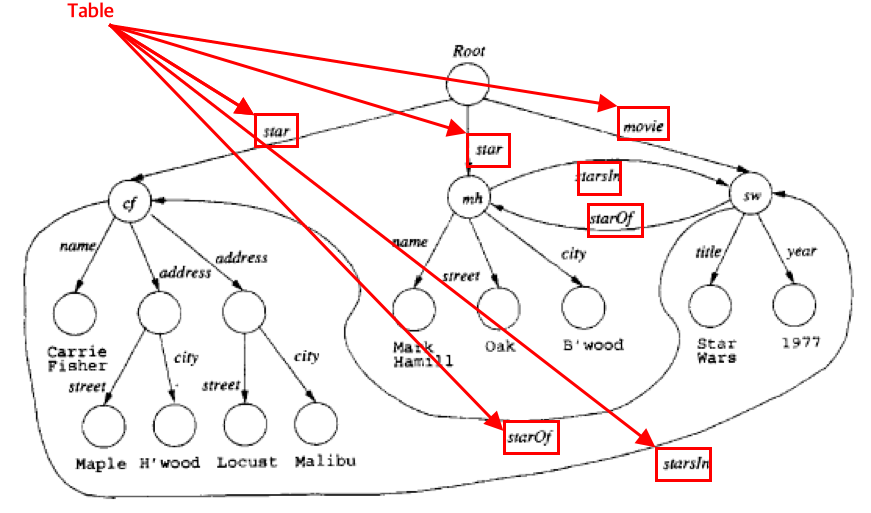
\includegraphics[width=\linewidth]{images/worksheet_9_solution_1.png}
            \end{center}

            \begin{center}
            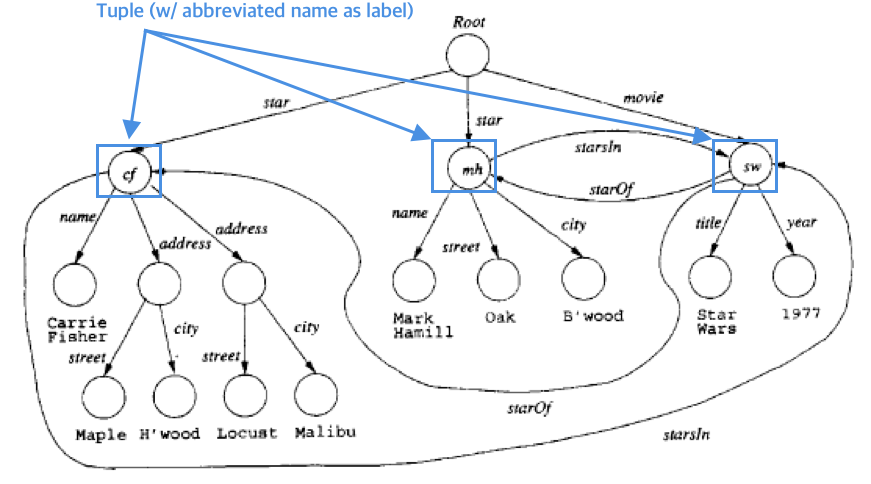
\includegraphics[width=\linewidth]{images/worksheet_9_solution_2.png}
            \end{center}

            \begin{center}
            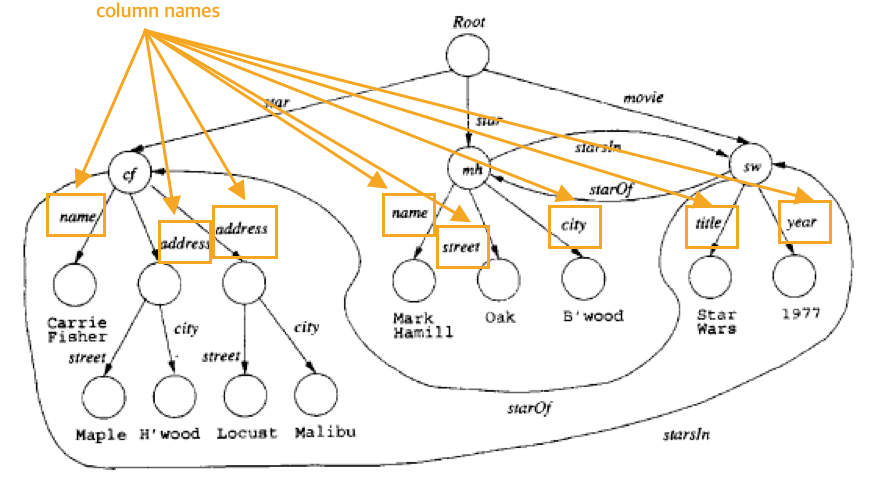
\includegraphics[width=\linewidth]{images/worksheet_9_solution_3.png}
            \end{center}

            \end{itemize}

            \item
        \end{itemize}

        \item

    \begin{center}
    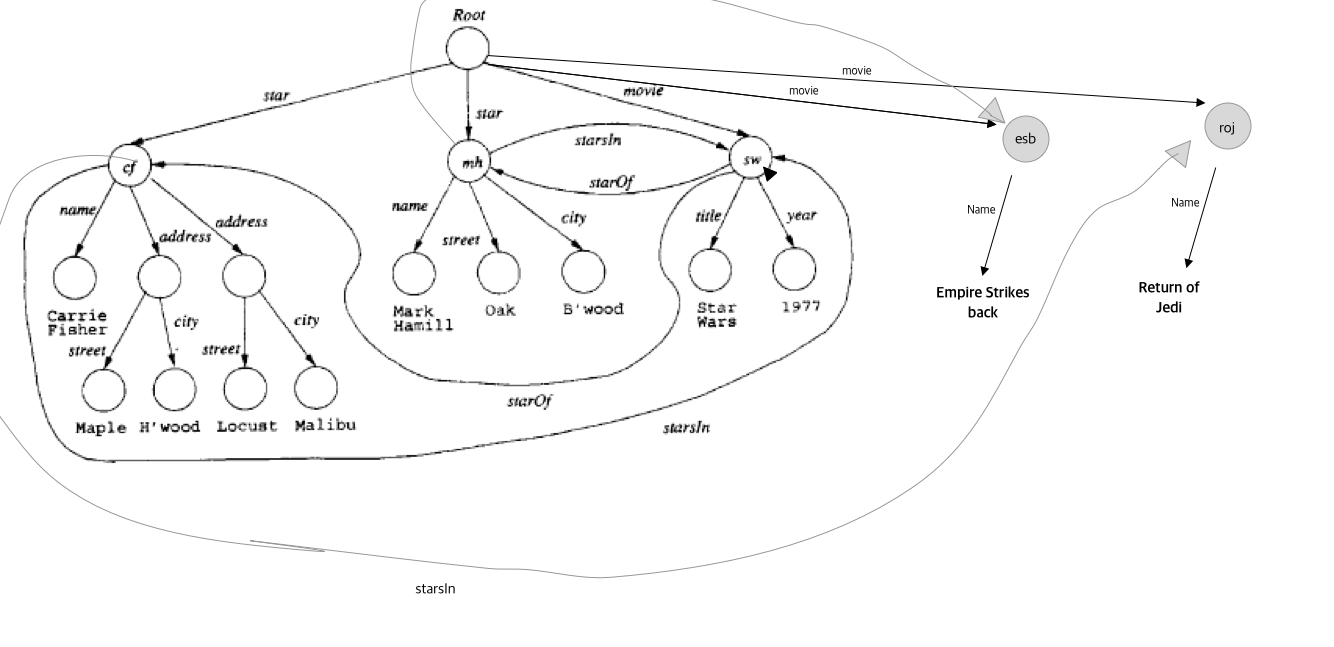
\includegraphics[width=\linewidth]{images/worksheet_9_solution_5.png}
    \end{center}


        \item

    \begin{center}
    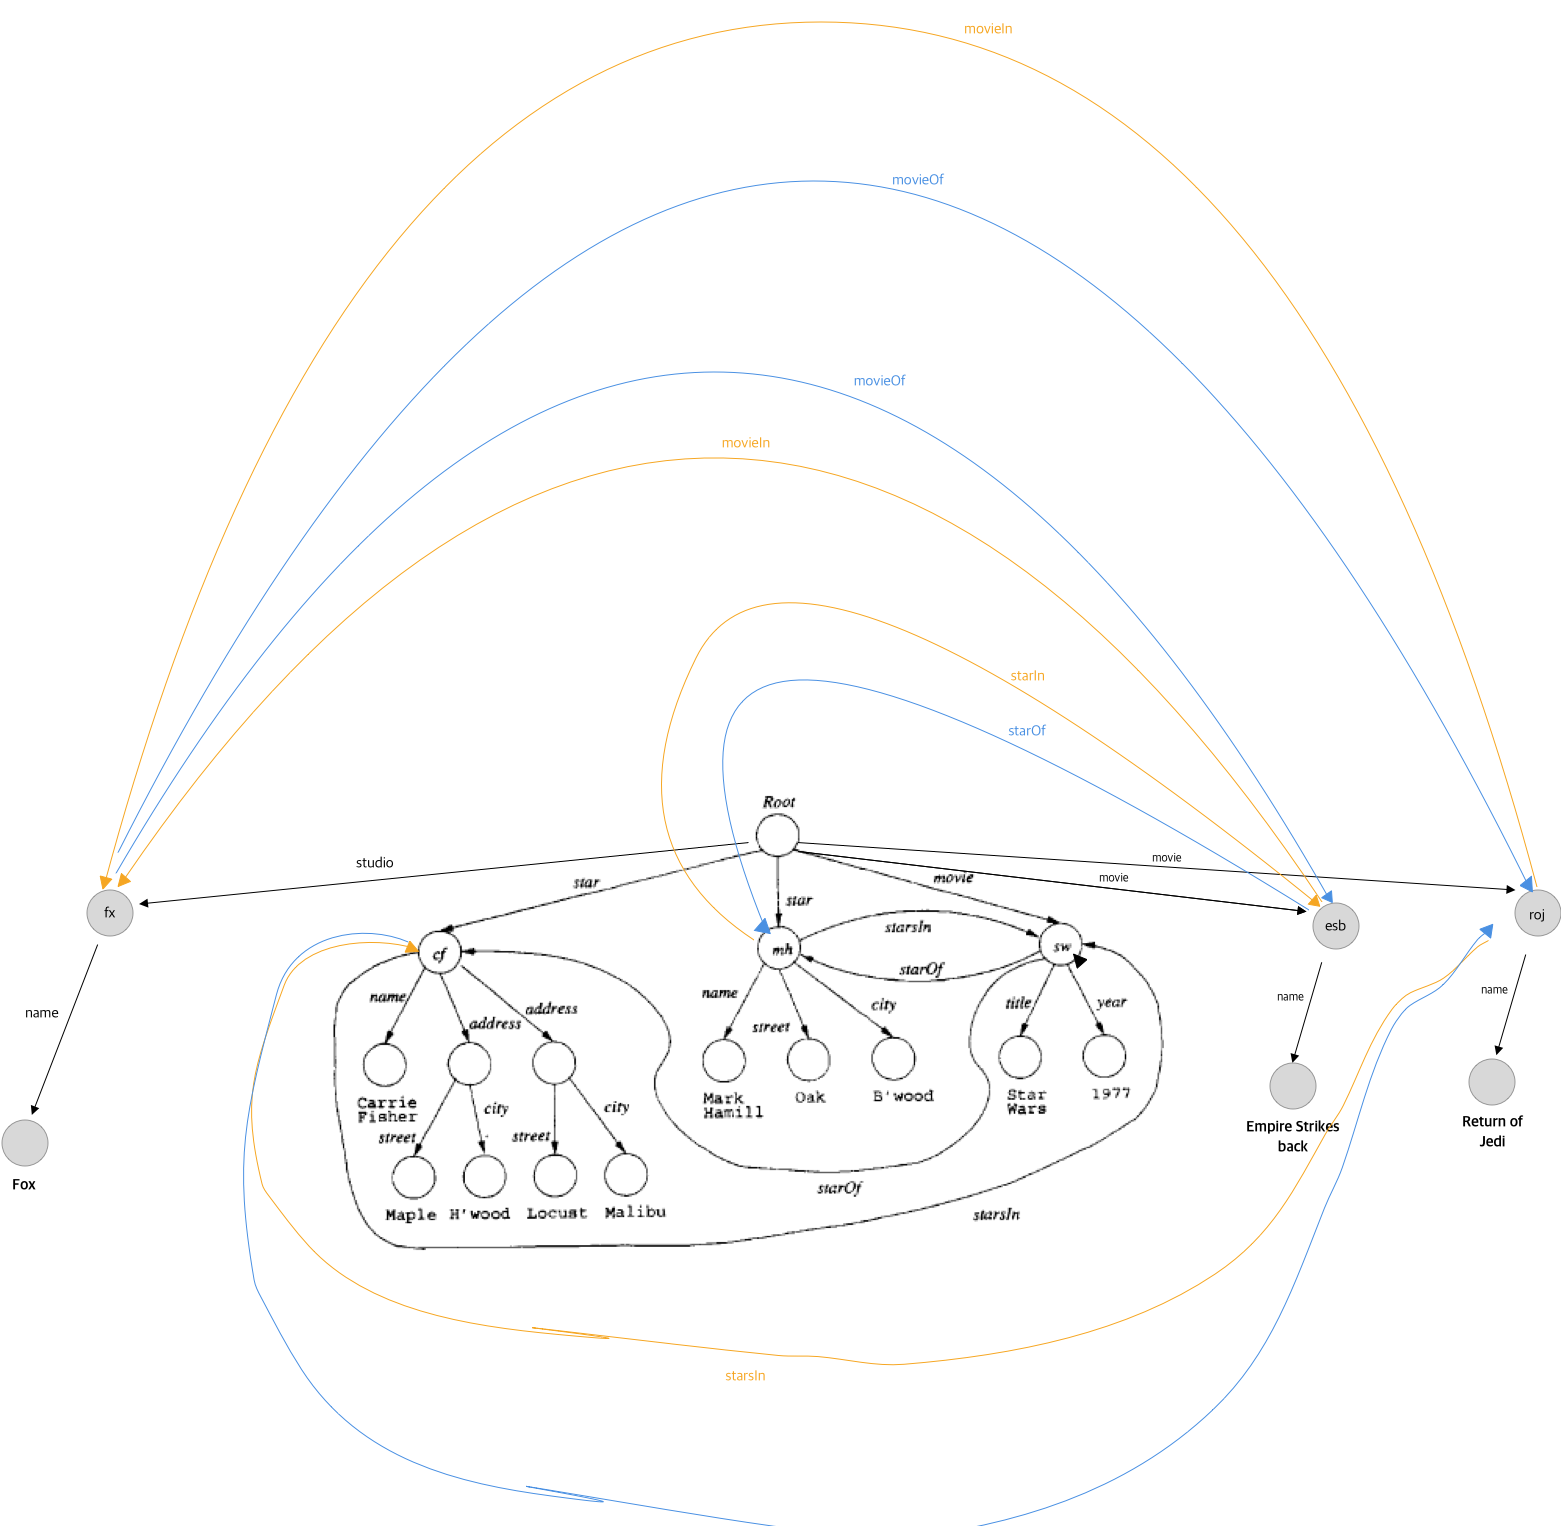
\includegraphics[width=\linewidth]{images/worksheet_9_solution_6.png}
    \end{center}

    \end{enumerate}

    \item

    \begin{center}
    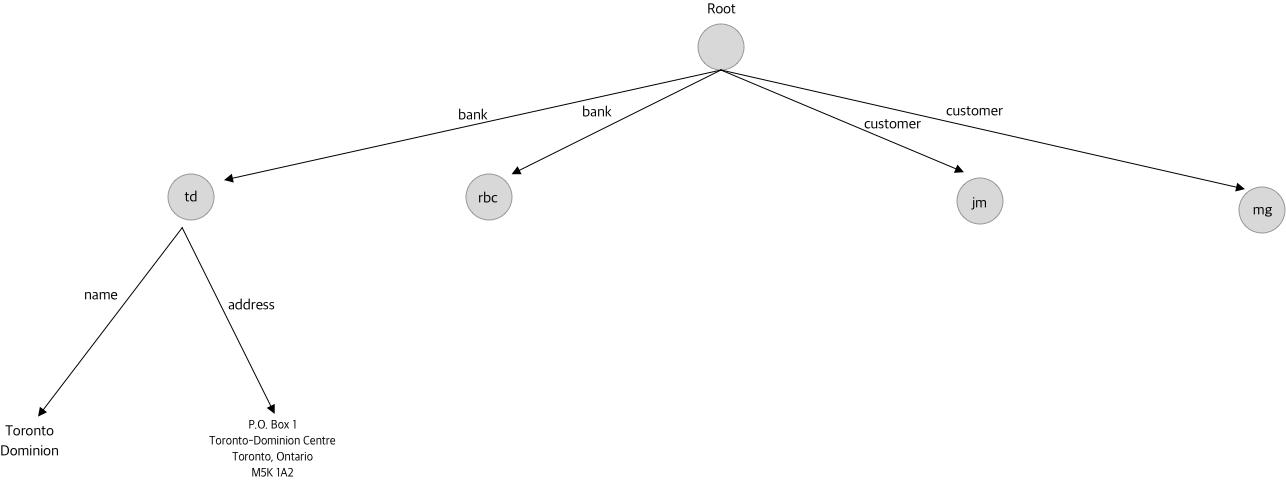
\includegraphics[width=\linewidth]{images/worksheet_9_solution_7.png}
    \end{center}

    \item

    \begin{center}
    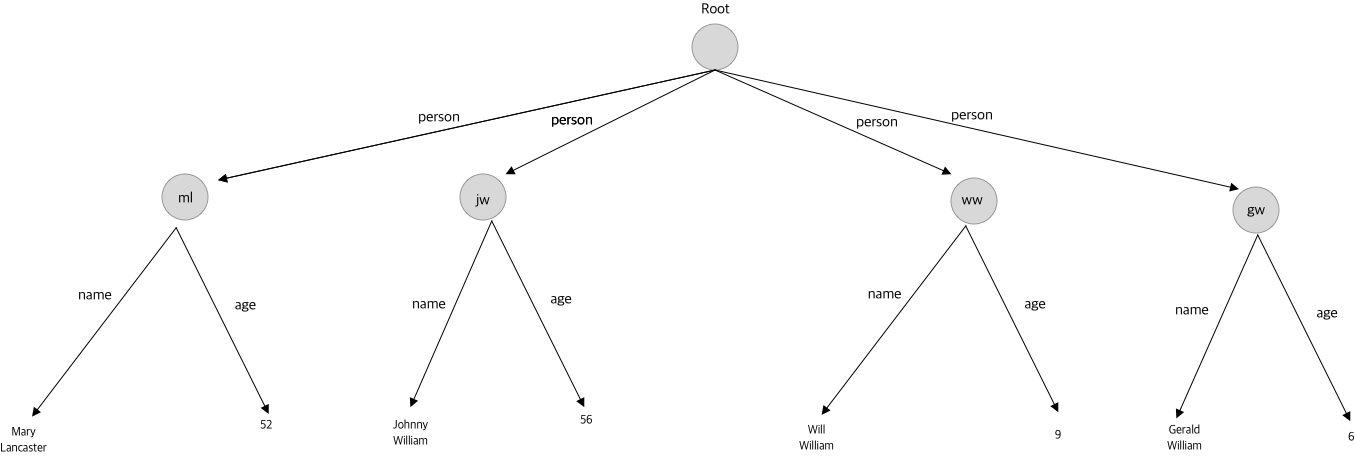
\includegraphics[width=\linewidth]{images/worksheet_9_solution_8.png}
    \end{center}

    \item

    The difference is that UML must fit data into its schema, where as the semi
    structured data allows whatever schema information that is appropriate to be attached to data

    \bigskip

    \underline{\textbf{Notees:}}

    \bigskip

    \begin{itemize}
        \item Semi-structured Data
        \begin{itemize}
            \item Is schemaless
            \item Is motivated primarily by its flexibility
            \item One could enter data at will, and attach to the data whatever schema information
            you felt was appropriate for that data.
            \item Makes query processing harder
        \end{itemize}
        \item Structured Data
        \begin{itemize}
            \item Is rigid framework into which data is placed.
            \item Data must fit into schema
            \item Fixed schema allows data to be organized with data structures
            that support efficient answering of queries
            \item e.g. UML, E/R, Relational, ODL
        \end{itemize}
    \end{itemize}

    \item

    \begin{enumerate}[a)]
        \item

    \begin{lstlisting}[language=XML]
    <? xml version = "1.0" encoding="utf-8" standalone = "yes">
    <StarMovieData>
        <Star starID="cf" starredIn="sw">
            <Name>Carrie Fisher</Name>
            <Address>
                <Street>123 Maple St.</Street>
                <City>Hollywood</City>
            </Address>
            <Address>
                <Street>5 Locust Ln.</Street>
                <City>Malibu</City>
            </Address>
        </Star>
        <Star starID="mh" starredIn="sw">
            <Name>Mark Hamill</Name>
            <Street>456 Oak Rd.</Street>
            <City>Brentwood</City>
        </Star>
        <Movie movieID="sw" starsOf="cf", "mh">
            <Title>Star Wars</Title>
            <Year>1977</Year>
        </Movie>
        <MovieExec movieExecID="gl" execsIn="sw">
            <Name>George Lucas</Name>
            <Position>Director</Position>
        </MovieExec>
        <MovieExec movieExecID="gk" execsIn="sw">
            <Name>Gru Kurtz</Name>
            <Position>Produced By</Position>
        </MovieExec>
    </StarMovieData>
    \end{lstlisting}

        \bigskip

    \begin{itemize}
        \item XML
        \begin{itemize}
            \item is called \textit{Extensible Markup Language}
            \item is an example of semistructured data
        \end{itemize}
        \item XML with and without a Schema
        \begin{itemize}
            \item has two different types
            \begin{enumerate}[1.]
                \item Well-formed XML
                \begin{itemize}
                    \item allows to invent your own tags
                    \item corresponds very-similarly to semi-structured data
                \end{itemize}

                \bigskip

                \underline{\textbf{Example:}}

                \bigskip

    \begin{lstlisting}[language=XML]
    <? xml version = "1.0" encoding="utf-8" standalone = "yes">
    <StarMovieData>
        <Star>
            <Name>Carrie Fisher</Name>
            <Address>
                <Street>123 Maple St.</Street>
                <City>Hollywood</City>
            </Address>
            <Address>
                <Street>5 Locust Ln.</Street>
                <City>Malibu</City>
            </Address>
        </Star>
        <Star>
            <Name>Mark Hamill</Name>
            <Street>456 Oak Rd.</Street>
            <City>Brentwood</City>
        </Star>
        <Movie>
            <Title>Star Wars</Title>
            <Year>1977</Year>
        </Movie>
    </StarMovieData>
    \end{lstlisting}

                \item Valid XML

                \begin{itemize}
                    \item Involes "Document Type Definition"
                    \item specifies allowable tags and gives a grammar for how they may be nested
                \end{itemize}

                \bigskip

            \end{enumerate}
        \end{itemize}

        \item Attributes
        \begin{itemize}
            \item is used to represent connections in a semistructured data graph

            \bigskip

            \underline{\textbf{Example:}}

            \bigskip

    \begin{lstlisting}[language=XML]
    <? xml version = "1.0" encoding="utf-8" standalone = "yes">
    <StarMovieData>
        <Star starID="cf" starredIn="sw">
            <Name>Carrie Fisher</Name>
            <Address>
                <Street>123 Maple St.</Street>
                <City>Hollywood</City>
            </Address>
            <Address>
                <Street>5 Locust Ln.</Street>
                <City>Malibu</City>
            </Address>
        </Star>
        <Star starID="mh" starredIn="sw">
            <Name>Mark Hamill</Name>
            <Street>456 Oak Rd.</Street>
            <City>Brentwood</City>
        </Star>
        <Movie starID="sw" starOf="cf", "mh">
            <Title>Star Wars</Title>
            <Year>1977</Year>
        </Movie>
    </StarMovieData>
    \end{lstlisting}

        \end{itemize}

        \item Namespaces
        \begin{itemize}
            \item \textbf{Syntax:} xmlns:\textit{name}:URI
            \item Is similar to import numpy as np in python
            \item Is used to distinguish tags coming from different sources, i.e. HTML

            \bigskip

            \underline{\textbf{Example:}}

            \bigskip

            Retireving element \textit{StarMovieData} from document \textbf{infolab.stanford.edu/movies}.
            Set md as the name of import

    \begin{lstlisting}[language=XML]
    <md:StarMovieData xmlns:md="http://infolab.stanford.edu/movies">
    \end{lstlisting}
        \end{itemize}
    \end{itemize}

        \item

    \begin{lstlisting}[language=XML]
    <? xml version = "1.0" encoding="utf-8" standalone = "yes">
    <StarMovieData>
        <Star starID="cf" starredIn="sw">
            <Name>Carrie Fisher</Name>
            <Address>
                <Street>123 Maple St.</Street>
                <City>Hollywood</City>
            </Address>
            <Address>
                <Street>5 Locust Ln.</Street>
                <City>Malibu</City>
            </Address>
        </Star>
        <Star starID="mh" starredIn="sw">
            <Name>Mark Hamill</Name>
            <Street>456 Oak Rd.</Street>
            <City>Brentwood</City>
        </Star>
        <Movie movieID="sw" starsOf="cf", "mh">
            <Title>Star Wars</Title>
            <Year>1977</Year>
        </Movie>
        <Movie movieID="esb" starOf="cf", "mh">
            <Title>Empire Strikes Back</Title>
            <Year>1980</Year>
        </Movie>
        <Movie movieID="roj" starOf="cf", "mh">
            <Title>Return of Jedi</Title>
            <Year>1983</Year>
        </Movie>
    </StarMovieData>
    \end{lstlisting}

    \end{enumerate}

\end{enumerate}

\end{document}